\documentclass[t]{beamer}
\usetheme{iclpt}
\nonstopmode

\author{Robert Kruszewski}
\title[Accelerating agent-based Python models]{Accelerating agent-based Python models}

\usepackage[T1]{fontenc}
\usepackage{lmodern}
\usepackage{tabularx, alltt, amsmath, multirow, graphicx, url, graphics, caption, natbib, listings, fancyhdr, lstlinebgrd, etoolbox, todonotes, colortbl}

\lstdefinelanguage[GNU99]{C}[99]{C}
  {morekeywords={asm,__asm__,__extension__,typeof,__typeof__}%
  }%

\lstdefinelanguage[99]{C}%
  {morekeywords={_Bool,_Complex,_Imaginary,auto,break,case,char,%
      const,continue,default,do,double,else,enum,extern,float,for,%
      goto,if,inline,int,long,register,restrict,return,short,signed,%
      sizeof,static,struct,switch,typedef,union,unsigned,void,volatile,%
      while},%
   sensitive,%
   morecomment=[s]{/*}{*/},%
   morecomment=[l]//,%
   morestring=[b]",%
   morestring=[b]',%
   moredelim=*[directive]\#,%
   moredirectives={define,elif,else,endif,error,if,ifdef,ifndef,line,%
      include,pragma,undef,warning}%
  }[keywords,comments,strings,directives]%

\definecolor{lightgray}{rgb}{0.83, 0.83, 0.83}
\definecolor{gray}{rgb}{0.5, 0.5, 0.5}
\definecolor{white}{rgb}{1, 1, 1}
\definecolor{lightcarminepink}{rgb}{0.9, 0.4, 0.38}
\definecolor{babyblue}{rgb}{0.54, 0.81, 0.94}

\lstset{
  basicstyle=\ttfamily,                   % Code font, Examples: \footnotesize, \ttfamily
  keywordstyle=\color{lightcarminepink},        % Keywords font ('*' = uppercase)
  commentstyle=\color{gray},              % Comments font
  numbers=left,                           % Line nums position
  numberstyle=\small\color{gray},                      % Line-numbers fonts
  stepnumber=1,                           % Step between two line-numbers
  numbersep=8pt,                          % How far are line-numbers from code
  backgroundcolor=\color{white}, % Choose background color
  frame=l,
  framerule=1.8pt,                             % A frame around the code
  xleftmargin=0em,
  framexleftmargin=1.7em,
  tabsize=4,                              % Default tab size
  captionpos=t,                           % Caption-position = bottom
  breaklines=true,                        % Automatic line breaking?
  breakatwhitespace=false,                % Automatic breaks only at whitespace?
  showspaces=false,                       % Dont make spaces visible
  showtabs=false,                         % Dont make tabls visible
  columns=fullflexible,                       % Column format
}

\begin{document}
\frame{\maketitle}

\begin{frame}
\frametitle{\huge Ecosystem modelling}
\begin{itemize}
	\item Metamodel
	\item Model
	\item Environment
\end{itemize}
\end{frame}


\begin{frame}[c]

\begin{center}
{\fontsize{48pt}{1em}\selectfont DEMO}
\end{center}

\end{frame}


\begin{frame}
\frametitle{VEW vs Fluidity}
\Large Virtual Ecology Workbench (VEW) \normalsize
\begin{itemize}
	\item One-dimensional physical environment.
	\item Uses Planktonica (DSL) for model specification.
	\item Widely tested and optimised
\end{itemize}
\vspace{12pt}
\Large Fluidity \normalsize
\begin{itemize}
	\item Three-dimensional environment
	\item Uses Python for model specification
	\item Gives VEW complain results, defies optimisation
\end{itemize}
% # Begin with DEMO

% ## THIS HAS TO TAKE 2 MINUTES (RECORD VIDEO OF SIMULATIONS)
% 1. Start a version that takes exactly 2 minutes and start speaking
% 2. Talk about VEW and 1D physics -> why Fluidity is a better solution for the future
% 3. Fluidity is slow - really slow -> Why?
% 4. We have a more sophisticated system but cannot use it in practice
% 5. Can we solve it -> probably, here's a possible solution that works
% 6. It can be done better -> why no one did?
% 7. Launch the same simulation as in point 1. but optimised so they both finish at the same time

% # Describe VEW and Fluidity (2-3 slides tops)
% ## What are the differences

\end{frame}


\begin{frame}[c]

\begin{figure}[H]
  \begin{center}
    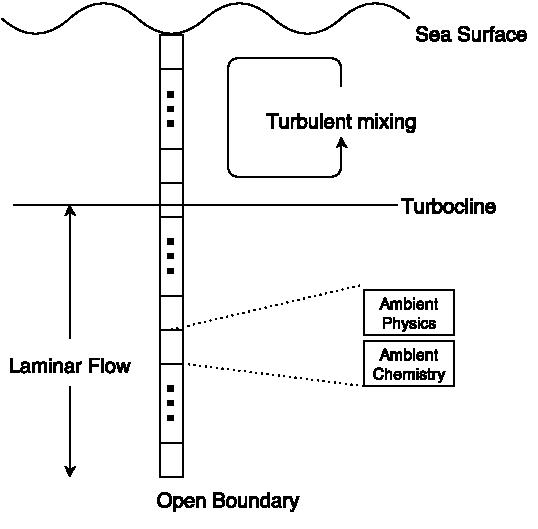
\includegraphics[width=0.6\textwidth,natwidth=473,natheight=466]{images/env-diagram.pdf}
  \end{center}
\end{figure}

\end{frame}


\begin{frame}[c]

\begin{figure}[H]
  \begin{center}
    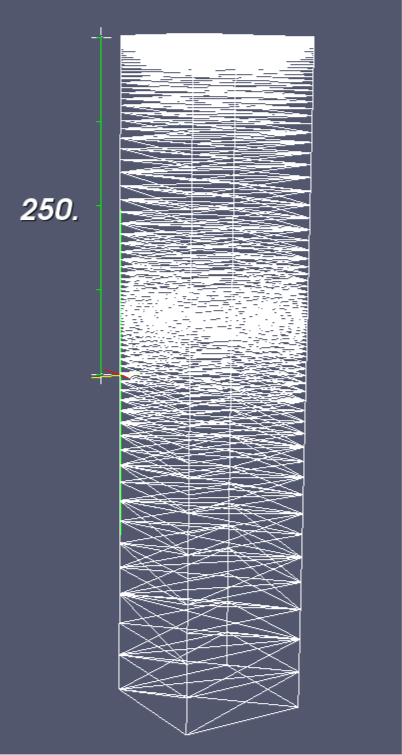
\includegraphics[height=0.9\textheight,natwidth=402,natheight=755]{images/fluidity-mesh.jpg}
  \end{center}
\end{figure}

\end{frame}

\begin{frame}[fragile,c]
\frametitle{\huge Challenge}
\begin{lstlisting}[
	language=python,
	caption=Python version
]
  Q_N = (vars['Ammonium'] + vars['AmmoniumIngested'] + vars['Nitrate'] + vars['NitrateIngested']) / vars['Carbon']
\end{lstlisting}

\begin{lstlisting}[
	language=c,
	caption=C version
]
float Q_N = (vars[AMMONIUM_POOL]) + vars[AMMONIUM_ING] + vars[NITRATE_POOL] + vars[NITRATE_ING]) / vars[CARBON_POOL];
\end{lstlisting}

\end{frame}


\begin{frame}[fragile,c]

\frametitle{\huge Python embedding}
\begin{lstlisting}[language=c]
#include <Python.h>
#include "modulename.h"

void cython_call() {
    Py_Initialize();
    initmodulename();
    ... call functions from "modulenam"
    Py_Finalize();
}
\end{lstlisting}

\end{frame}

\begin{frame}[fragile,c]

\frametitle{\huge Array wrappers}
\begin{lstlisting}[language=python]
cdef class AgentWrapper:

    cdef float * array

    def __getitem__(self, key):
        return self.array[agentNames[key]]

    def __setitem__(self, key, value):
        self.array[agentNames[key]] = value
\end{lstlisting}
\end{frame}


\begin{frame}[c]

\begin{figure}[ht!]
  \begin{center}
    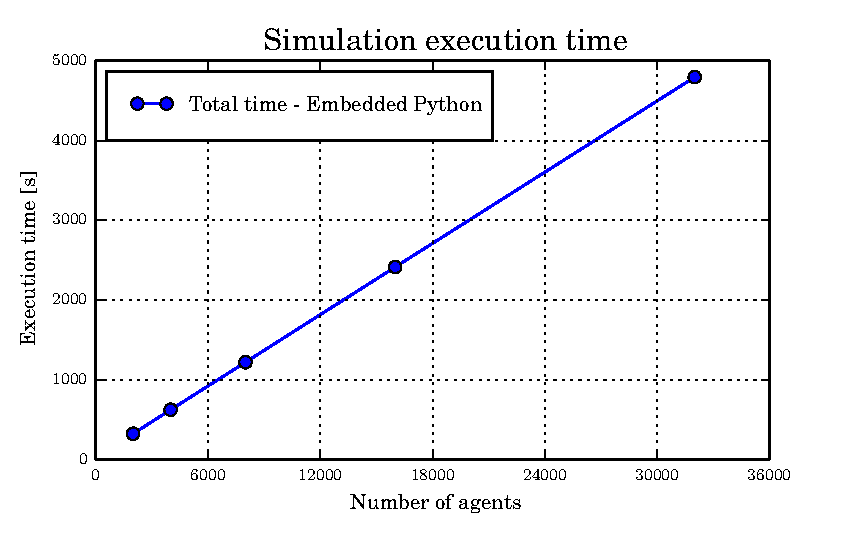
\includegraphics[width=\columnwidth]{graphs/cython-perf.eps}
  \end{center}
\end{figure}

\end{frame}


\begin{frame}[c]

\begin{figure}[ht!]
  \begin{center}
    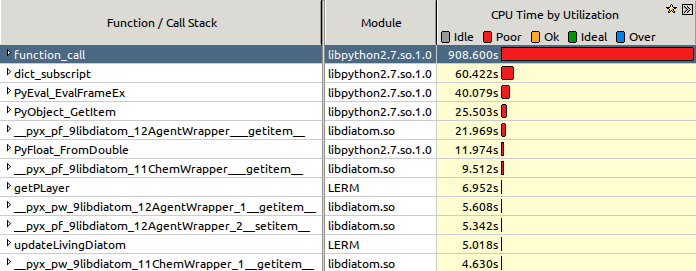
\includegraphics[width=\textwidth,natwidth=696,natheight=271]{images/vtune-cython-pure.png}
  \end{center}
\end{figure}

\end{frame}


\begin{frame}[c]

\begin{center}
{\fontsize{60pt}{1em}\selectfont Thank you}
\end{center}

\end{frame}


\begin{frame}[c]

\begin{center}
{\fontsize{48pt}{1em}\selectfont Questions?}
\end{center}

\end{frame}

\end{document}
